\documentclass[1p]{elsarticle_modified}
%\bibliographystyle{elsarticle-num}

%\usepackage[colorlinks]{hyperref}
%\usepackage{abbrmath_seonhwa} %\Abb, \Ascr, \Acal ,\Abf, \Afrak
\usepackage{amsfonts}
\usepackage{amssymb}
\usepackage{amsmath}
\usepackage{amsthm}
\usepackage{scalefnt}
\usepackage{amsbsy}
\usepackage{kotex}
\usepackage{caption}
\usepackage{subfig}
\usepackage{color}
\usepackage{graphicx}
\usepackage{xcolor} %% white, black, red, green, blue, cyan, magenta, yellow
\usepackage{float}
\usepackage{setspace}
\usepackage{hyperref}

\usepackage{tikz}
\usetikzlibrary{arrows}

\usepackage{multirow}
\usepackage{array} % fixed length table
\usepackage{hhline}

%%%%%%%%%%%%%%%%%%%%%
\makeatletter
\renewcommand*\env@matrix[1][\arraystretch]{%
	\edef\arraystretch{#1}%
	\hskip -\arraycolsep
	\let\@ifnextchar\new@ifnextchar
	\array{*\c@MaxMatrixCols c}}
\makeatother %https://tex.stackexchange.com/questions/14071/how-can-i-increase-the-line-spacing-in-a-matrix
%%%%%%%%%%%%%%%

\usepackage[normalem]{ulem}

\newcommand{\msout}[1]{\ifmmode\text{\sout{\ensuremath{#1}}}\else\sout{#1}\fi}
%SOURCE: \msout is \stkout macro in https://tex.stackexchange.com/questions/20609/strikeout-in-math-mode

\newcommand{\cancel}[1]{
	\ifmmode
	{\color{red}\msout{#1}}
	\else
	{\color{red}\sout{#1}}
	\fi
}

\newcommand{\add}[1]{
	{\color{blue}\uwave{#1}}
}

\newcommand{\replace}[2]{
	\ifmmode
	{\color{red}\msout{#1}}{\color{blue}\uwave{#2}}
	\else
	{\color{red}\sout{#1}}{\color{blue}\uwave{#2}}
	\fi
}

\newcommand{\Sol}{\mathcal{S}} %segment
\newcommand{\D}{D} %diagram
\newcommand{\A}{\mathcal{A}} %arc


%%%%%%%%%%%%%%%%%%%%%%%%%%%%%5 test

\def\sl{\operatorname{\textup{SL}}(2,\Cbb)}
\def\psl{\operatorname{\textup{PSL}}(2,\Cbb)}
\def\quan{\mkern 1mu \triangleright \mkern 1mu}

\theoremstyle{definition}
\newtheorem{thm}{Theorem}[section]
\newtheorem{prop}[thm]{Proposition}
\newtheorem{lem}[thm]{Lemma}
\newtheorem{ques}[thm]{Question}
\newtheorem{cor}[thm]{Corollary}
\newtheorem{defn}[thm]{Definition}
\newtheorem{exam}[thm]{Example}
\newtheorem{rmk}[thm]{Remark}
\newtheorem{alg}[thm]{Algorithm}

\newcommand{\I}{\sqrt{-1}}
\begin{document}

%\begin{frontmatter}
%
%\title{Boundary parabolic representations of knots up to 8 crossings}
%
%%% Group authors per affiliation:
%\author{Yunhi Cho} 
%\address{Department of Mathematics, University of Seoul, Seoul, Korea}
%\ead{yhcho@uos.ac.kr}
%
%
%\author{Seonhwa Kim} %\fnref{s_kim}}
%\address{Center for Geometry and Physics, Institute for Basic Science, Pohang, 37673, Korea}
%\ead{ryeona17@ibs.re.kr}
%
%\author{Hyuk Kim}
%\address{Department of Mathematical Sciences, Seoul National University, Seoul 08826, Korea}
%\ead{hyukkim@snu.ac.kr}
%
%\author{Seokbeom Yoon}
%\address{Department of Mathematical Sciences, Seoul National University, Seoul, 08826,  Korea}
%\ead{sbyoon15@snu.ac.kr}
%
%\begin{abstract}
%We find all boundary parabolic representation of knots up to 8 crossings.
%
%\end{abstract}
%\begin{keyword}
%    \MSC[2010] 57M25 
%\end{keyword}
%
%\end{frontmatter}

%\linenumbers
%\tableofcontents
%
\newcommand\colored[1]{\textcolor{white}{\rule[-0.35ex]{0.8em}{1.4ex}}\kern-0.8em\color{red} #1}%
%\newcommand\colored[1]{\textcolor{white}{ #1}\kern-2.17ex	\textcolor{white}{ #1}\kern-1.81ex	\textcolor{white}{ #1}\kern-2.15ex\color{red}#1	}

{\Large $\underline{12a_{0191}~(K12a_{0191})}$}

\setlength{\tabcolsep}{10pt}
\renewcommand{\arraystretch}{1.6}
\vspace{1cm}\begin{tabular}{m{100pt}>{\centering\arraybackslash}m{274pt}}
\multirow{5}{120pt}{
	\centering
	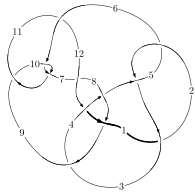
\includegraphics[width=112pt]{../../../GIT/diagram.site/Diagrams/png/992_12a_0191.png}\\
\ \ \ A knot diagram\footnotemark}&
\allowdisplaybreaks
\textbf{Linearized knot diagam} \\
\cline{2-2}
 &
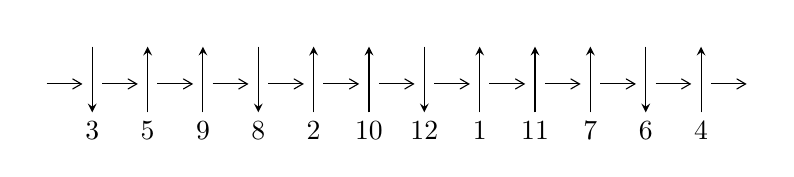
\begin{tikzpicture}[x=20pt, y=17pt]
	% nodes
	\node (C0) at (0, 0) {};
	\node (C1) at (1, 0) {};
	\node (C1U) at (1, +1) {};
	\node (C1D) at (1, -1) {3};

	\node (C2) at (2, 0) {};
	\node (C2U) at (2, +1) {};
	\node (C2D) at (2, -1) {5};

	\node (C3) at (3, 0) {};
	\node (C3U) at (3, +1) {};
	\node (C3D) at (3, -1) {9};

	\node (C4) at (4, 0) {};
	\node (C4U) at (4, +1) {};
	\node (C4D) at (4, -1) {8};

	\node (C5) at (5, 0) {};
	\node (C5U) at (5, +1) {};
	\node (C5D) at (5, -1) {2};

	\node (C6) at (6, 0) {};
	\node (C6U) at (6, +1) {};
	\node (C6D) at (6, -1) {10};

	\node (C7) at (7, 0) {};
	\node (C7U) at (7, +1) {};
	\node (C7D) at (7, -1) {12};

	\node (C8) at (8, 0) {};
	\node (C8U) at (8, +1) {};
	\node (C8D) at (8, -1) {1};

	\node (C9) at (9, 0) {};
	\node (C9U) at (9, +1) {};
	\node (C9D) at (9, -1) {11};

	\node (C10) at (10, 0) {};
	\node (C10U) at (10, +1) {};
	\node (C10D) at (10, -1) {7};

	\node (C11) at (11, 0) {};
	\node (C11U) at (11, +1) {};
	\node (C11D) at (11, -1) {6};

	\node (C12) at (12, 0) {};
	\node (C12U) at (12, +1) {};
	\node (C12D) at (12, -1) {4};
	\node (C13) at (13, 0) {};

	% arrows
	\draw[->,>={angle 60}]
	(C0) edge (C1) (C1) edge (C2) (C2) edge (C3) (C3) edge (C4) (C4) edge (C5) (C5) edge (C6) (C6) edge (C7) (C7) edge (C8) (C8) edge (C9) (C9) edge (C10) (C10) edge (C11) (C11) edge (C12) (C12) edge (C13) ;	\draw[->,>=stealth]
	(C1U) edge (C1D) (C2D) edge (C2U) (C3D) edge (C3U) (C4U) edge (C4D) (C5D) edge (C5U) (C6D) edge (C6U) (C7U) edge (C7D) (C8D) edge (C8U) (C9D) edge (C9U) (C10D) edge (C10U) (C11U) edge (C11D) (C12D) edge (C12U) ;
	\end{tikzpicture} \\
\hhline{~~} \\& 
\textbf{Solving Sequence} \\ \cline{2-2} 
 &
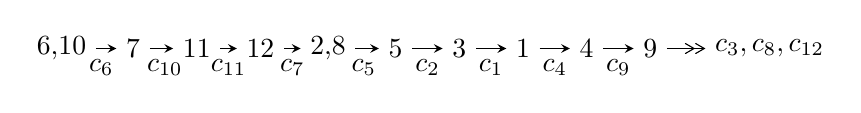
\begin{tikzpicture}[x=23pt, y=7pt]
	% node
	\node (A0) at (-1/8, 0) {6,10};
	\node (A1) at (1, 0) {7};
	\node (A2) at (2, 0) {11};
	\node (A3) at (3, 0) {12};
	\node (A4) at (65/16, 0) {2,8};
	\node (A5) at (41/8, 0) {5};
	\node (A6) at (49/8, 0) {3};
	\node (A7) at (57/8, 0) {1};
	\node (A8) at (65/8, 0) {4};
	\node (A9) at (73/8, 0) {9};
	\node (C1) at (1/2, -1) {$c_{6}$};
	\node (C2) at (3/2, -1) {$c_{10}$};
	\node (C3) at (5/2, -1) {$c_{11}$};
	\node (C4) at (7/2, -1) {$c_{7}$};
	\node (C5) at (37/8, -1) {$c_{5}$};
	\node (C6) at (45/8, -1) {$c_{2}$};
	\node (C7) at (53/8, -1) {$c_{1}$};
	\node (C8) at (61/8, -1) {$c_{4}$};
	\node (C9) at (69/8, -1) {$c_{9}$};
	\node (A10) at (11, 0) {$c_{3},c_{8},c_{12}$};

	% edge
	\draw[->,>=stealth]	
	(A0) edge (A1) (A1) edge (A2) (A2) edge (A3) (A3) edge (A4) (A4) edge (A5) (A5) edge (A6) (A6) edge (A7) (A7) edge (A8) (A8) edge (A9) ;
	\draw[->>,>={angle 60}]	
	(A9) edge (A10);
\end{tikzpicture} \\ 

\end{tabular} \\

\footnotetext{
The image of knot diagram is generated by the software ``\textbf{Draw programme}" developed by Andrew Bartholomew(\url{http://www.layer8.co.uk/maths/draw/index.htm\#Running-draw}), where we modified some parts for our purpose(\url{https://github.com/CATsTAILs/LinksPainter}).
}\phantom \\ \newline 
\centering \textbf{Ideals for irreducible components\footnotemark of $X_{\text{par}}$} 
 
\begin{align*}
I^u_{1}&=\langle 
2.52008\times10^{86} u^{132}+3.94249\times10^{86} u^{131}+\cdots+2.40447\times10^{86} b+4.48441\times10^{86},\\
\phantom{I^u_{1}}&\phantom{= \langle  }8.35432\times10^{85} u^{132}+1.84786\times10^{86} u^{131}+\cdots+3.00559\times10^{85} a+5.71468\times10^{85},\;u^{133}+3 u^{132}+\cdots+8 u+1\rangle \\
I^u_{2}&=\langle 
b^2- b+1,\;a+1,\;u+1\rangle \\
\\
\end{align*}
\raggedright * 2 irreducible components of $\dim_{\mathbb{C}}=0$, with total 135 representations.\\
\footnotetext{All coefficients of polynomials are rational numbers. But the coefficients are sometimes approximated in decimal forms when there is not enough margin.}
\newpage
\renewcommand{\arraystretch}{1}
\centering \section*{I. $I^u_{1}= \langle 2.52\times10^{86} u^{132}+3.94\times10^{86} u^{131}+\cdots+2.40\times10^{86} b+4.48\times10^{86},\;8.35\times10^{85} u^{132}+1.85\times10^{86} u^{131}+\cdots+3.01\times10^{85} a+5.71\times10^{85},\;u^{133}+3 u^{132}+\cdots+8 u+1 \rangle$}
\flushleft \textbf{(i) Arc colorings}\\
\begin{tabular}{m{7pt} m{180pt} m{7pt} m{180pt} }
\flushright $a_{6}=$&$\begin{pmatrix}1\\0\end{pmatrix}$ \\
\flushright $a_{10}=$&$\begin{pmatrix}0\\u\end{pmatrix}$ \\
\flushright $a_{7}=$&$\begin{pmatrix}1\\- u^2\end{pmatrix}$ \\
\flushright $a_{11}=$&$\begin{pmatrix}u\\- u^3+u\end{pmatrix}$ \\
\flushright $a_{12}=$&$\begin{pmatrix}u^3\\- u^3+u\end{pmatrix}$ \\
\flushright $a_{2}=$&$\begin{pmatrix}-2.77960 u^{132}-6.14809 u^{131}+\cdots-19.5449 u-1.90135\\-1.04808 u^{132}-1.63965 u^{131}+\cdots-12.4583 u-1.86503\end{pmatrix}$ \\
\flushright $a_{8}=$&$\begin{pmatrix}u^8- u^6+u^4+1\\- u^8+2 u^6-2 u^4\end{pmatrix}$ \\
\flushright $a_{5}=$&$\begin{pmatrix}-1.55645 u^{132}-7.01862 u^{131}+\cdots-38.9986 u-5.29904\\-0.441377 u^{132}-0.416986 u^{131}+\cdots-7.60203 u-2.08587\end{pmatrix}$ \\
\flushright $a_{3}=$&$\begin{pmatrix}-2.59310 u^{132}-8.40110 u^{131}+\cdots-48.5351 u-7.64213\\0.250137 u^{132}+1.15429 u^{131}+\cdots-2.41571 u-1.48573\end{pmatrix}$ \\
\flushright $a_{1}=$&$\begin{pmatrix}4.12887 u^{132}+9.16088 u^{131}+\cdots+36.0661 u+3.95573\\1.59710 u^{132}+4.52162 u^{131}+\cdots+17.3842 u+2.23057\end{pmatrix}$ \\
\flushright $a_{4}=$&$\begin{pmatrix}4.25425 u^{132}+6.02863 u^{131}+\cdots+0.864270 u-0.604074\\-4.48777 u^{132}-9.82783 u^{131}+\cdots-40.5969 u-6.76622\end{pmatrix}$ \\
\flushright $a_{9}=$&$\begin{pmatrix}- u^3\\u^5- u^3+u\end{pmatrix}$\\&\end{tabular}
\flushleft \textbf{(ii) Obstruction class $= -1$}\\~\\
\flushleft \textbf{(iii) Cusp Shapes $= 12.1017 u^{132}+39.4347 u^{131}+\cdots+227.831 u+41.4535$}\\~\\
\newpage\renewcommand{\arraystretch}{1}
\flushleft \textbf{(iv) u-Polynomials at the component}\newline \\
\begin{tabular}{m{50pt}|m{274pt}}
Crossings & \hspace{64pt}u-Polynomials at each crossing \\
\hline $$\begin{aligned}c_{1}\end{aligned}$$&$\begin{aligned}
&u^{133}+56 u^{132}+\cdots-31 u-1
\end{aligned}$\\
\hline $$\begin{aligned}c_{2},c_{5}\end{aligned}$$&$\begin{aligned}
&u^{133}+2 u^{132}+\cdots-3 u-1
\end{aligned}$\\
\hline $$\begin{aligned}c_{3}\end{aligned}$$&$\begin{aligned}
&u^{133}+2 u^{132}+\cdots-51 u-1
\end{aligned}$\\
\hline $$\begin{aligned}c_{4}\end{aligned}$$&$\begin{aligned}
&u^{133}+4 u^{132}+\cdots-503 u-71
\end{aligned}$\\
\hline $$\begin{aligned}c_{6},c_{10}\end{aligned}$$&$\begin{aligned}
&u^{133}-3 u^{132}+\cdots+8 u-1
\end{aligned}$\\
\hline $$\begin{aligned}c_{7}\end{aligned}$$&$\begin{aligned}
&u^{133}- u^{132}+\cdots+149316216 u-14182609
\end{aligned}$\\
\hline $$\begin{aligned}c_{8}\end{aligned}$$&$\begin{aligned}
&u^{133}-7 u^{132}+\cdots+4 u^2-1
\end{aligned}$\\
\hline $$\begin{aligned}c_{9}\end{aligned}$$&$\begin{aligned}
&u^{133}-63 u^{132}+\cdots+8 u-1
\end{aligned}$\\
\hline $$\begin{aligned}c_{11}\end{aligned}$$&$\begin{aligned}
&u^{133}-3 u^{132}+\cdots+149248 u-14144
\end{aligned}$\\
\hline $$\begin{aligned}c_{12}\end{aligned}$$&$\begin{aligned}
&u^{133}+13 u^{132}+\cdots+4 u-4
\end{aligned}$\\
\hline
\end{tabular}\\~\\
\newpage\renewcommand{\arraystretch}{1}
\flushleft \textbf{(v) Riley Polynomials at the component}\newline \\
\begin{tabular}{m{50pt}|m{274pt}}
Crossings & \hspace{64pt}Riley Polynomials at each crossing \\
\hline $$\begin{aligned}c_{1}\end{aligned}$$&$\begin{aligned}
&y^{133}+44 y^{132}+\cdots-463 y-1
\end{aligned}$\\
\hline $$\begin{aligned}c_{2},c_{5}\end{aligned}$$&$\begin{aligned}
&y^{133}+56 y^{132}+\cdots-31 y-1
\end{aligned}$\\
\hline $$\begin{aligned}c_{3}\end{aligned}$$&$\begin{aligned}
&y^{133}-144 y^{132}+\cdots+469 y-1
\end{aligned}$\\
\hline $$\begin{aligned}c_{4}\end{aligned}$$&$\begin{aligned}
&y^{133}-148 y^{132}+\cdots+609145 y-5041
\end{aligned}$\\
\hline $$\begin{aligned}c_{6},c_{10}\end{aligned}$$&$\begin{aligned}
&y^{133}-63 y^{132}+\cdots+8 y-1
\end{aligned}$\\
\hline $$\begin{aligned}c_{7}\end{aligned}$$&$\begin{aligned}
&y^{133}-55 y^{132}+\cdots+8218121135689976 y-201146398046881
\end{aligned}$\\
\hline $$\begin{aligned}c_{8}\end{aligned}$$&$\begin{aligned}
&y^{133}-15 y^{132}+\cdots+8 y-1
\end{aligned}$\\
\hline $$\begin{aligned}c_{9}\end{aligned}$$&$\begin{aligned}
&y^{133}+17 y^{132}+\cdots-188 y-1
\end{aligned}$\\
\hline $$\begin{aligned}c_{11}\end{aligned}$$&$\begin{aligned}
&y^{133}+23 y^{132}+\cdots-6938136960 y-200052736
\end{aligned}$\\
\hline $$\begin{aligned}c_{12}\end{aligned}$$&$\begin{aligned}
&y^{133}+15 y^{132}+\cdots-376 y-16
\end{aligned}$\\
\hline
\end{tabular}\\~\\
\newpage\flushleft \textbf{(vi) Complex Volumes and Cusp Shapes}
$$\begin{array}{c|c|c}  
\text{Solutions to }I^u_{1}& \I (\text{vol} + \sqrt{-1}CS) & \text{Cusp shape}\\
 \hline 
\begin{aligned}
u &= -0.938642 + 0.337279 I \\
a &= \phantom{-}0.20985 - 2.16393 I \\
b &= \phantom{-}0.390528 - 0.825680 I\end{aligned}
 & \phantom{-}1.30397 - 2.83605 I & \phantom{-0.000000 } 0 \\ \hline\begin{aligned}
u &= -0.938642 - 0.337279 I \\
a &= \phantom{-}0.20985 + 2.16393 I \\
b &= \phantom{-}0.390528 + 0.825680 I\end{aligned}
 & \phantom{-}1.30397 + 2.83605 I & \phantom{-0.000000 } 0 \\ \hline\begin{aligned}
u &= \phantom{-}0.676793 + 0.700478 I \\
a &= \phantom{-}1.40666 - 1.02355 I \\
b &= -0.420429 - 1.023560 I\end{aligned}
 & -5.04185 + 3.41791 I & \phantom{-0.000000 } 0 \\ \hline\begin{aligned}
u &= \phantom{-}0.676793 - 0.700478 I \\
a &= \phantom{-}1.40666 + 1.02355 I \\
b &= -0.420429 + 1.023560 I\end{aligned}
 & -5.04185 - 3.41791 I & \phantom{-0.000000 } 0 \\ \hline\begin{aligned}
u &= -0.628150 + 0.722355 I \\
a &= \phantom{-}1.21898 + 1.37771 I \\
b &= -0.631474 + 1.133740 I\end{aligned}
 & -3.83179 - 11.75880 I & \phantom{-0.000000 } 0 \\ \hline\begin{aligned}
u &= -0.628150 - 0.722355 I \\
a &= \phantom{-}1.21898 - 1.37771 I \\
b &= -0.631474 - 1.133740 I\end{aligned}
 & -3.83179 + 11.75880 I & \phantom{-0.000000 } 0 \\ \hline\begin{aligned}
u &= \phantom{-}0.567642 + 0.770256 I \\
a &= \phantom{-}0.128927 + 0.853025 I \\
b &= -0.418769 + 1.003390 I\end{aligned}
 & -5.10093 - 2.87602 I & \phantom{-0.000000 } 0 \\ \hline\begin{aligned}
u &= \phantom{-}0.567642 - 0.770256 I \\
a &= \phantom{-}0.128927 - 0.853025 I \\
b &= -0.418769 - 1.003390 I\end{aligned}
 & -5.10093 + 2.87602 I & \phantom{-0.000000 } 0 \\ \hline\begin{aligned}
u &= -1.021260 + 0.272501 I \\
a &= -5.04520 - 0.52842 I \\
b &= \phantom{-}0.529033 + 0.889780 I\end{aligned}
 & \phantom{-}2.01730 + 1.36993 I & \phantom{-0.000000 } 0 \\ \hline\begin{aligned}
u &= -1.021260 - 0.272501 I \\
a &= -5.04520 + 0.52842 I \\
b &= \phantom{-}0.529033 - 0.889780 I\end{aligned}
 & \phantom{-}2.01730 - 1.36993 I & \phantom{-0.000000 } 0\\
 \hline 
 \end{array}$$\newpage$$\begin{array}{c|c|c}  
\text{Solutions to }I^u_{1}& \I (\text{vol} + \sqrt{-1}CS) & \text{Cusp shape}\\
 \hline 
\begin{aligned}
u &= -0.619041 + 0.690475 I \\
a &= -0.045587 + 0.329564 I \\
b &= -0.869286 - 0.403020 I\end{aligned}
 & -1.64002 - 6.22274 I & \phantom{-0.000000 } 0 \\ \hline\begin{aligned}
u &= -0.619041 - 0.690475 I \\
a &= -0.045587 - 0.329564 I \\
b &= -0.869286 + 0.403020 I\end{aligned}
 & -1.64002 + 6.22274 I & \phantom{-0.000000 } 0 \\ \hline\begin{aligned}
u &= -1.033370 + 0.306485 I \\
a &= -3.13350 + 3.70534 I \\
b &= \phantom{-}0.529045 - 0.819274 I\end{aligned}
 & \phantom{-}2.24662 - 2.89797 I & \phantom{-0.000000 } 0 \\ \hline\begin{aligned}
u &= -1.033370 - 0.306485 I \\
a &= -3.13350 - 3.70534 I \\
b &= \phantom{-}0.529045 + 0.819274 I\end{aligned}
 & \phantom{-}2.24662 + 2.89797 I & \phantom{-0.000000 } 0 \\ \hline\begin{aligned}
u &= \phantom{-}0.447619 + 0.798125 I \\
a &= \phantom{-}0.353224 - 0.921347 I \\
b &= -0.327771 - 0.941641 I\end{aligned}
 & -4.45007 - 0.29957 I & \phantom{-0.000000 } 0 \\ \hline\begin{aligned}
u &= \phantom{-}0.447619 - 0.798125 I \\
a &= \phantom{-}0.353224 + 0.921347 I \\
b &= -0.327771 + 0.941641 I\end{aligned}
 & -4.45007 + 0.29957 I & \phantom{-0.000000 } 0 \\ \hline\begin{aligned}
u &= \phantom{-}1.073510 + 0.162208 I \\
a &= \phantom{-}0.112836 + 0.745408 I \\
b &= \phantom{-}0.006446 - 1.247370 I\end{aligned}
 & -1.89384 - 3.73566 I & \phantom{-0.000000 } 0 \\ \hline\begin{aligned}
u &= \phantom{-}1.073510 - 0.162208 I \\
a &= \phantom{-}0.112836 - 0.745408 I \\
b &= \phantom{-}0.006446 + 1.247370 I\end{aligned}
 & -1.89384 + 3.73566 I & \phantom{-0.000000 } 0 \\ \hline\begin{aligned}
u &= \phantom{-}1.061100 + 0.243227 I \\
a &= -1.74905 + 1.01661 I \\
b &= \phantom{-}0.688737 - 1.162250 I\end{aligned}
 & \phantom{-}2.81853 - 3.85336 I & \phantom{-0.000000 } 0 \\ \hline\begin{aligned}
u &= \phantom{-}1.061100 - 0.243227 I \\
a &= -1.74905 - 1.01661 I \\
b &= \phantom{-}0.688737 + 1.162250 I\end{aligned}
 & \phantom{-}2.81853 + 3.85336 I & \phantom{-0.000000 } 0\\
 \hline 
 \end{array}$$\newpage$$\begin{array}{c|c|c}  
\text{Solutions to }I^u_{1}& \I (\text{vol} + \sqrt{-1}CS) & \text{Cusp shape}\\
 \hline 
\begin{aligned}
u &= \phantom{-}0.906727 + 0.616271 I \\
a &= \phantom{-}0.099342 + 0.230960 I \\
b &= -0.350822 + 1.034860 I\end{aligned}
 & -4.35526 + 1.63876 I & \phantom{-0.000000 } 0 \\ \hline\begin{aligned}
u &= \phantom{-}0.906727 - 0.616271 I \\
a &= \phantom{-}0.099342 - 0.230960 I \\
b &= -0.350822 - 1.034860 I\end{aligned}
 & -4.35526 - 1.63876 I & \phantom{-0.000000 } 0 \\ \hline\begin{aligned}
u &= -1.058580 + 0.286836 I \\
a &= \phantom{-}0.498544 - 0.542479 I \\
b &= \phantom{-}0.124828 + 0.188943 I\end{aligned}
 & \phantom{-}2.30068 - 0.56140 I & \phantom{-0.000000 } 0 \\ \hline\begin{aligned}
u &= -1.058580 - 0.286836 I \\
a &= \phantom{-}0.498544 + 0.542479 I \\
b &= \phantom{-}0.124828 - 0.188943 I\end{aligned}
 & \phantom{-}2.30068 + 0.56140 I & \phantom{-0.000000 } 0 \\ \hline\begin{aligned}
u &= \phantom{-}1.019480 + 0.424090 I \\
a &= -0.817365 - 0.136498 I \\
b &= \phantom{-}0.297876 + 1.126390 I\end{aligned}
 & \phantom{-}0.24508 + 5.65314 I & \phantom{-0.000000 } 0 \\ \hline\begin{aligned}
u &= \phantom{-}1.019480 - 0.424090 I \\
a &= -0.817365 + 0.136498 I \\
b &= \phantom{-}0.297876 - 1.126390 I\end{aligned}
 & \phantom{-}0.24508 - 5.65314 I & \phantom{-0.000000 } 0 \\ \hline\begin{aligned}
u &= -0.550163 + 0.704374 I \\
a &= -0.14235 - 1.45370 I \\
b &= -0.099381 - 1.260370 I\end{aligned}
 & -7.42423 - 3.38928 I & \phantom{-0.000000 } 0 \\ \hline\begin{aligned}
u &= -0.550163 - 0.704374 I \\
a &= -0.14235 + 1.45370 I \\
b &= -0.099381 + 1.260370 I\end{aligned}
 & -7.42423 + 3.38928 I & \phantom{-0.000000 } 0 \\ \hline\begin{aligned}
u &= \phantom{-}1.071030 + 0.283668 I \\
a &= -1.77636 + 1.17552 I \\
b &= \phantom{-}0.954457 - 0.590743 I\end{aligned}
 & \phantom{-}4.97036 - 1.30489 I & \phantom{-0.000000 } 0 \\ \hline\begin{aligned}
u &= \phantom{-}1.071030 - 0.283668 I \\
a &= -1.77636 - 1.17552 I \\
b &= \phantom{-}0.954457 + 0.590743 I\end{aligned}
 & \phantom{-}4.97036 + 1.30489 I & \phantom{-0.000000 } 0\\
 \hline 
 \end{array}$$\newpage$$\begin{array}{c|c|c}  
\text{Solutions to }I^u_{1}& \I (\text{vol} + \sqrt{-1}CS) & \text{Cusp shape}\\
 \hline 
\begin{aligned}
u &= \phantom{-}0.341275 + 0.823182 I \\
a &= \phantom{-}1.22741 + 0.72538 I \\
b &= -0.517719 + 1.008110 I\end{aligned}
 & -3.16841 - 6.11783 I & \phantom{-0.000000 } 0 \\ \hline\begin{aligned}
u &= \phantom{-}0.341275 - 0.823182 I \\
a &= \phantom{-}1.22741 - 0.72538 I \\
b &= -0.517719 - 1.008110 I\end{aligned}
 & -3.16841 + 6.11783 I & \phantom{-0.000000 } 0 \\ \hline\begin{aligned}
u &= \phantom{-}1.057330 + 0.345227 I \\
a &= -2.41464 - 0.92687 I \\
b &= \phantom{-}0.776115 + 1.029020 I\end{aligned}
 & \phantom{-}3.65902 + 4.97237 I & \phantom{-0.000000 } 0 \\ \hline\begin{aligned}
u &= \phantom{-}1.057330 - 0.345227 I \\
a &= -2.41464 + 0.92687 I \\
b &= \phantom{-}0.776115 - 1.029020 I\end{aligned}
 & \phantom{-}3.65902 - 4.97237 I & \phantom{-0.000000 } 0 \\ \hline\begin{aligned}
u &= \phantom{-}1.071840 + 0.310160 I \\
a &= -1.76398 - 0.47056 I \\
b &= \phantom{-}0.948474 + 0.360859 I\end{aligned}
 & \phantom{-}5.19875 + 2.12290 I & \phantom{-0.000000 } 0 \\ \hline\begin{aligned}
u &= \phantom{-}1.071840 - 0.310160 I \\
a &= -1.76398 + 0.47056 I \\
b &= \phantom{-}0.948474 - 0.360859 I\end{aligned}
 & \phantom{-}5.19875 - 2.12290 I & \phantom{-0.000000 } 0 \\ \hline\begin{aligned}
u &= -0.365567 + 0.804751 I \\
a &= \phantom{-}1.25879 - 1.05621 I \\
b &= -0.663331 - 1.142380 I\end{aligned}
 & -2.4075 + 14.5311 I & \phantom{-0.000000 } 0 \\ \hline\begin{aligned}
u &= -0.365567 - 0.804751 I \\
a &= \phantom{-}1.25879 + 1.05621 I \\
b &= -0.663331 + 1.142380 I\end{aligned}
 & -2.4075 - 14.5311 I & \phantom{-0.000000 } 0 \\ \hline\begin{aligned}
u &= -0.812176 + 0.318124 I \\
a &= \phantom{-}1.47266 + 0.35071 I \\
b &= \phantom{-}0.215975 + 0.502125 I\end{aligned}
 & \phantom{-}1.029600 - 0.175314 I & \phantom{-0.000000 } 0 \\ \hline\begin{aligned}
u &= -0.812176 - 0.318124 I \\
a &= \phantom{-}1.47266 - 0.35071 I \\
b &= \phantom{-}0.215975 - 0.502125 I\end{aligned}
 & \phantom{-}1.029600 + 0.175314 I & \phantom{-0.000000 } 0\\
 \hline 
 \end{array}$$\newpage$$\begin{array}{c|c|c}  
\text{Solutions to }I^u_{1}& \I (\text{vol} + \sqrt{-1}CS) & \text{Cusp shape}\\
 \hline 
\begin{aligned}
u &= -0.956485 + 0.601189 I \\
a &= \phantom{-}0.881721 + 0.725739 I \\
b &= -0.825847 + 0.376564 I\end{aligned}
 & -0.641585 + 1.245630 I & \phantom{-0.000000 } 0 \\ \hline\begin{aligned}
u &= -0.956485 - 0.601189 I \\
a &= \phantom{-}0.881721 - 0.725739 I \\
b &= -0.825847 - 0.376564 I\end{aligned}
 & -0.641585 - 1.245630 I & \phantom{-0.000000 } 0 \\ \hline\begin{aligned}
u &= -0.359356 + 0.784698 I \\
a &= \phantom{-}0.190011 - 0.403009 I \\
b &= -0.922850 + 0.445182 I\end{aligned}
 & -0.28125 + 8.72203 I & \phantom{-0.000000 } 0 \\ \hline\begin{aligned}
u &= -0.359356 - 0.784698 I \\
a &= \phantom{-}0.190011 + 0.403009 I \\
b &= -0.922850 - 0.445182 I\end{aligned}
 & -0.28125 - 8.72203 I & \phantom{-0.000000 } 0 \\ \hline\begin{aligned}
u &= -0.401720 + 0.758509 I \\
a &= -0.267477 + 1.249090 I \\
b &= -0.038805 + 1.300870 I\end{aligned}
 & -6.66241 + 5.90589 I & \phantom{-0.000000 } 0 \\ \hline\begin{aligned}
u &= -0.401720 - 0.758509 I \\
a &= -0.267477 - 1.249090 I \\
b &= -0.038805 - 1.300870 I\end{aligned}
 & -6.66241 - 5.90589 I & \phantom{-0.000000 } 0 \\ \hline\begin{aligned}
u &= \phantom{-}0.560497 + 0.648811 I \\
a &= \phantom{-}0.524922 - 0.403750 I \\
b &= -0.424723 + 0.078114 I\end{aligned}
 & -2.73017 + 0.09703 I & \phantom{-0.000000 } 0 \\ \hline\begin{aligned}
u &= \phantom{-}0.560497 - 0.648811 I \\
a &= \phantom{-}0.524922 + 0.403750 I \\
b &= -0.424723 - 0.078114 I\end{aligned}
 & -2.73017 - 0.09703 I & \phantom{-0.000000 } 0 \\ \hline\begin{aligned}
u &= -0.960239 + 0.633625 I \\
a &= -0.0716142 - 0.1064080 I \\
b &= -0.612797 - 1.124860 I\end{aligned}
 & -2.84776 + 6.59074 I & \phantom{-0.000000 } 0 \\ \hline\begin{aligned}
u &= -0.960239 - 0.633625 I \\
a &= -0.0716142 + 0.1064080 I \\
b &= -0.612797 + 1.124860 I\end{aligned}
 & -2.84776 - 6.59074 I & \phantom{-0.000000 } 0\\
 \hline 
 \end{array}$$\newpage$$\begin{array}{c|c|c}  
\text{Solutions to }I^u_{1}& \I (\text{vol} + \sqrt{-1}CS) & \text{Cusp shape}\\
 \hline 
\begin{aligned}
u &= \phantom{-}1.000500 + 0.574022 I \\
a &= \phantom{-}0.745653 - 0.228474 I \\
b &= -0.510788 + 0.042986 I\end{aligned}
 & -1.43249 + 4.68363 I & \phantom{-0.000000 } 0 \\ \hline\begin{aligned}
u &= \phantom{-}1.000500 - 0.574022 I \\
a &= \phantom{-}0.745653 + 0.228474 I \\
b &= -0.510788 - 0.042986 I\end{aligned}
 & -1.43249 - 4.68363 I & \phantom{-0.000000 } 0 \\ \hline\begin{aligned}
u &= \phantom{-}1.139840 + 0.197666 I \\
a &= \phantom{-}1.73211 + 0.78820 I \\
b &= -0.899455 - 0.481249 I\end{aligned}
 & \phantom{-}4.53074 - 6.07300 I & \phantom{-0.000000 } 0 \\ \hline\begin{aligned}
u &= \phantom{-}1.139840 - 0.197666 I \\
a &= \phantom{-}1.73211 - 0.78820 I \\
b &= -0.899455 + 0.481249 I\end{aligned}
 & \phantom{-}4.53074 + 6.07300 I & \phantom{-0.000000 } 0 \\ \hline\begin{aligned}
u &= -1.032740 + 0.540075 I \\
a &= \phantom{-}0.959201 - 0.018023 I \\
b &= \phantom{-}0.495730 + 1.212150 I\end{aligned}
 & -0.589793 - 0.316757 I & \phantom{-0.000000 } 0 \\ \hline\begin{aligned}
u &= -1.032740 - 0.540075 I \\
a &= \phantom{-}0.959201 + 0.018023 I \\
b &= \phantom{-}0.495730 - 1.212150 I\end{aligned}
 & -0.589793 + 0.316757 I & \phantom{-0.000000 } 0 \\ \hline\begin{aligned}
u &= \phantom{-}1.157920 + 0.180871 I \\
a &= \phantom{-}1.88931 - 0.83451 I \\
b &= -0.668196 + 1.121420 I\end{aligned}
 & \phantom{-}2.58003 - 11.84430 I & \phantom{-0.000000 } 0 \\ \hline\begin{aligned}
u &= \phantom{-}1.157920 - 0.180871 I \\
a &= \phantom{-}1.88931 + 0.83451 I \\
b &= -0.668196 - 1.121420 I\end{aligned}
 & \phantom{-}2.58003 + 11.84430 I & \phantom{-0.000000 } 0 \\ \hline\begin{aligned}
u &= -1.014170 + 0.598205 I \\
a &= \phantom{-}1.64661 + 0.85587 I \\
b &= -0.136108 + 1.241100 I\end{aligned}
 & -6.05194 - 1.61446 I & \phantom{-0.000000 } 0 \\ \hline\begin{aligned}
u &= -1.014170 - 0.598205 I \\
a &= \phantom{-}1.64661 - 0.85587 I \\
b &= -0.136108 - 1.241100 I\end{aligned}
 & -6.05194 + 1.61446 I & \phantom{-0.000000 } 0\\
 \hline 
 \end{array}$$\newpage$$\begin{array}{c|c|c}  
\text{Solutions to }I^u_{1}& \I (\text{vol} + \sqrt{-1}CS) & \text{Cusp shape}\\
 \hline 
\begin{aligned}
u &= -1.186470 + 0.054021 I \\
a &= \phantom{-}1.189560 - 0.564974 I \\
b &= -0.431034 + 0.890623 I\end{aligned}
 & \phantom{-}1.13183 - 1.75913 I & \phantom{-0.000000 } 0 \\ \hline\begin{aligned}
u &= -1.186470 - 0.054021 I \\
a &= \phantom{-}1.189560 + 0.564974 I \\
b &= -0.431034 - 0.890623 I\end{aligned}
 & \phantom{-}1.13183 + 1.75913 I & \phantom{-0.000000 } 0 \\ \hline\begin{aligned}
u &= -0.516975 + 0.621794 I \\
a &= -0.50686 - 1.74873 I \\
b &= \phantom{-}0.558570 - 1.198940 I\end{aligned}
 & -2.11838 - 4.26875 I & \phantom{-}4.00000 + 8.90330 I \\ \hline\begin{aligned}
u &= -0.516975 - 0.621794 I \\
a &= -0.50686 + 1.74873 I \\
b &= \phantom{-}0.558570 + 1.198940 I\end{aligned}
 & -2.11838 + 4.26875 I & \phantom{-}4.00000 - 8.90330 I \\ \hline\begin{aligned}
u &= \phantom{-}0.326269 + 0.737922 I \\
a &= \phantom{-}0.581012 + 0.276327 I \\
b &= -0.384807 - 0.441827 I\end{aligned}
 & -1.67402 - 2.04228 I & \phantom{-0.000000 -}0. + 3.11343 I \\ \hline\begin{aligned}
u &= \phantom{-}0.326269 - 0.737922 I \\
a &= \phantom{-}0.581012 - 0.276327 I \\
b &= -0.384807 + 0.441827 I\end{aligned}
 & -1.67402 + 2.04228 I & \phantom{-0.000000 } 0. - 3.11343 I \\ \hline\begin{aligned}
u &= -1.164350 + 0.267658 I \\
a &= \phantom{-}1.57158 - 0.87908 I \\
b &= -0.431717 + 0.707305 I\end{aligned}
 & \phantom{-}2.69578 - 0.90782 I & \phantom{-0.000000 } 0 \\ \hline\begin{aligned}
u &= -1.164350 - 0.267658 I \\
a &= \phantom{-}1.57158 + 0.87908 I \\
b &= -0.431717 - 0.707305 I\end{aligned}
 & \phantom{-}2.69578 + 0.90782 I & \phantom{-0.000000 } 0 \\ \hline\begin{aligned}
u &= -1.073090 + 0.525884 I \\
a &= -0.02919 - 1.69397 I \\
b &= \phantom{-}0.855172 + 0.938845 I\end{aligned}
 & \phantom{-}2.42996 - 1.91167 I & \phantom{-0.000000 } 0 \\ \hline\begin{aligned}
u &= -1.073090 - 0.525884 I \\
a &= -0.02919 + 1.69397 I \\
b &= \phantom{-}0.855172 - 0.938845 I\end{aligned}
 & \phantom{-}2.42996 + 1.91167 I & \phantom{-0.000000 } 0\\
 \hline 
 \end{array}$$\newpage$$\begin{array}{c|c|c}  
\text{Solutions to }I^u_{1}& \I (\text{vol} + \sqrt{-1}CS) & \text{Cusp shape}\\
 \hline 
\begin{aligned}
u &= \phantom{-}1.056950 + 0.559305 I \\
a &= \phantom{-}0.10846 - 1.87568 I \\
b &= \phantom{-}0.430768 - 0.937711 I\end{aligned}
 & -0.51321 + 3.28432 I & \phantom{-0.000000 } 0 \\ \hline\begin{aligned}
u &= \phantom{-}1.056950 - 0.559305 I \\
a &= \phantom{-}0.10846 + 1.87568 I \\
b &= \phantom{-}0.430768 + 0.937711 I\end{aligned}
 & -0.51321 - 3.28432 I & \phantom{-0.000000 } 0 \\ \hline\begin{aligned}
u &= \phantom{-}0.464633 + 0.655641 I \\
a &= -1.26428 + 3.48917 I \\
b &= \phantom{-}0.458134 + 0.928503 I\end{aligned}
 & -2.25487 + 1.46344 I & \phantom{-}10.47361 + 7.88997 I \\ \hline\begin{aligned}
u &= \phantom{-}0.464633 - 0.655641 I \\
a &= -1.26428 - 3.48917 I \\
b &= \phantom{-}0.458134 - 0.928503 I\end{aligned}
 & -2.25487 - 1.46344 I & \phantom{-}10.47361 - 7.88997 I \\ \hline\begin{aligned}
u &= -0.376109 + 0.709583 I \\
a &= -1.00205 + 1.36804 I \\
b &= \phantom{-}0.644594 + 1.215780 I\end{aligned}
 & -1.43164 + 6.14743 I & \phantom{-}4.00000 - 9.28084 I \\ \hline\begin{aligned}
u &= -0.376109 - 0.709583 I \\
a &= -1.00205 - 1.36804 I \\
b &= \phantom{-}0.644594 - 1.215780 I\end{aligned}
 & -1.43164 - 6.14743 I & \phantom{-}4.00000 + 9.28084 I \\ \hline\begin{aligned}
u &= \phantom{-}1.013000 + 0.643963 I \\
a &= \phantom{-}1.54835 - 0.88471 I \\
b &= -0.452616 - 1.029990 I\end{aligned}
 & -3.77821 + 8.20381 I & \phantom{-0.000000 } 0 \\ \hline\begin{aligned}
u &= \phantom{-}1.013000 - 0.643963 I \\
a &= \phantom{-}1.54835 + 0.88471 I \\
b &= -0.452616 + 1.029990 I\end{aligned}
 & -3.77821 - 8.20381 I & \phantom{-0.000000 } 0 \\ \hline\begin{aligned}
u &= \phantom{-}0.407638 + 0.685721 I \\
a &= -2.80601 - 2.71556 I \\
b &= \phantom{-}0.506623 - 0.928041 I\end{aligned}
 & -1.98627 - 3.38011 I & \phantom{-}4.0000 - 16.6696 I \\ \hline\begin{aligned}
u &= \phantom{-}0.407638 - 0.685721 I \\
a &= -2.80601 + 2.71556 I \\
b &= \phantom{-}0.506623 + 0.928041 I\end{aligned}
 & -1.98627 + 3.38011 I & \phantom{-}4.0000 + 16.6696 I\\
 \hline 
 \end{array}$$\newpage$$\begin{array}{c|c|c}  
\text{Solutions to }I^u_{1}& \I (\text{vol} + \sqrt{-1}CS) & \text{Cusp shape}\\
 \hline 
\begin{aligned}
u &= \phantom{-}1.081200 + 0.545165 I \\
a &= -0.03586 + 3.05446 I \\
b &= \phantom{-}0.524517 - 0.749014 I\end{aligned}
 & \phantom{-}0.57689 + 3.95354 I & \phantom{-0.000000 } 0 \\ \hline\begin{aligned}
u &= \phantom{-}1.081200 - 0.545165 I \\
a &= -0.03586 - 3.05446 I \\
b &= \phantom{-}0.524517 + 0.749014 I\end{aligned}
 & \phantom{-}0.57689 - 3.95354 I & \phantom{-0.000000 } 0 \\ \hline\begin{aligned}
u &= \phantom{-}1.149370 + 0.396511 I \\
a &= \phantom{-}1.44488 - 1.33207 I \\
b &= -0.793011 + 0.596511 I\end{aligned}
 & \phantom{-}6.81136 + 5.77876 I & \phantom{-0.000000 } 0 \\ \hline\begin{aligned}
u &= \phantom{-}1.149370 - 0.396511 I \\
a &= \phantom{-}1.44488 + 1.33207 I \\
b &= -0.793011 - 0.596511 I\end{aligned}
 & \phantom{-}6.81136 - 5.77876 I & \phantom{-0.000000 } 0 \\ \hline\begin{aligned}
u &= -1.091750 + 0.535401 I \\
a &= -0.60127 - 1.63173 I \\
b &= \phantom{-}0.986693 + 0.216479 I\end{aligned}
 & \phantom{-}3.67042 - 5.02818 I & \phantom{-0.000000 } 0 \\ \hline\begin{aligned}
u &= -1.091750 - 0.535401 I \\
a &= -0.60127 + 1.63173 I \\
b &= \phantom{-}0.986693 - 0.216479 I\end{aligned}
 & \phantom{-}3.67042 + 5.02818 I & \phantom{-0.000000 } 0 \\ \hline\begin{aligned}
u &= \phantom{-}1.091490 + 0.541216 I \\
a &= -0.281364 - 0.569955 I \\
b &= \phantom{-}0.268631 + 0.463462 I\end{aligned}
 & \phantom{-}0.58808 + 6.56631 I & \phantom{-0.000000 } 0 \\ \hline\begin{aligned}
u &= \phantom{-}1.091490 - 0.541216 I \\
a &= -0.281364 + 0.569955 I \\
b &= \phantom{-}0.268631 - 0.463462 I\end{aligned}
 & \phantom{-}0.58808 - 6.56631 I & \phantom{-0.000000 } 0 \\ \hline\begin{aligned}
u &= -1.201860 + 0.200635 I \\
a &= \phantom{-}1.54186 + 0.83855 I \\
b &= -0.514690 - 0.951900 I\end{aligned}
 & \phantom{-}1.86540 + 3.13414 I & \phantom{-0.000000 } 0 \\ \hline\begin{aligned}
u &= -1.201860 - 0.200635 I \\
a &= \phantom{-}1.54186 - 0.83855 I \\
b &= -0.514690 + 0.951900 I\end{aligned}
 & \phantom{-}1.86540 - 3.13414 I & \phantom{-0.000000 } 0\\
 \hline 
 \end{array}$$\newpage$$\begin{array}{c|c|c}  
\text{Solutions to }I^u_{1}& \I (\text{vol} + \sqrt{-1}CS) & \text{Cusp shape}\\
 \hline 
\begin{aligned}
u &= \phantom{-}1.084700 + 0.562327 I \\
a &= -4.28667 + 1.91345 I \\
b &= \phantom{-}0.524320 + 0.933011 I\end{aligned}
 & -0.00612 + 8.20949 I & \phantom{-0.000000 } 0 \\ \hline\begin{aligned}
u &= \phantom{-}1.084700 - 0.562327 I \\
a &= -4.28667 - 1.91345 I \\
b &= \phantom{-}0.524320 - 0.933011 I\end{aligned}
 & -0.00612 - 8.20949 I & \phantom{-0.000000 } 0 \\ \hline\begin{aligned}
u &= -1.097070 + 0.548031 I \\
a &= -2.18238 - 0.84343 I \\
b &= \phantom{-}0.987094 - 0.694444 I\end{aligned}
 & \phantom{-}3.18188 - 8.50354 I & \phantom{-0.000000 } 0 \\ \hline\begin{aligned}
u &= -1.097070 - 0.548031 I \\
a &= -2.18238 + 0.84343 I \\
b &= \phantom{-}0.987094 + 0.694444 I\end{aligned}
 & \phantom{-}3.18188 + 8.50354 I & \phantom{-0.000000 } 0 \\ \hline\begin{aligned}
u &= -1.098860 + 0.564154 I \\
a &= -2.84194 - 0.95940 I \\
b &= \phantom{-}0.669594 - 1.231270 I\end{aligned}
 & \phantom{-}0.67683 - 11.03360 I & \phantom{-0.000000 } 0 \\ \hline\begin{aligned}
u &= -1.098860 - 0.564154 I \\
a &= -2.84194 + 0.95940 I \\
b &= \phantom{-}0.669594 + 1.231270 I\end{aligned}
 & \phantom{-}0.67683 + 11.03360 I & \phantom{-0.000000 } 0 \\ \hline\begin{aligned}
u &= -1.150740 + 0.453999 I \\
a &= \phantom{-}2.31207 + 0.01912 I \\
b &= -0.720083 + 0.655606 I\end{aligned}
 & \phantom{-}6.42598 - 2.29873 I & \phantom{-0.000000 } 0 \\ \hline\begin{aligned}
u &= -1.150740 - 0.453999 I \\
a &= \phantom{-}2.31207 - 0.01912 I \\
b &= -0.720083 - 0.655606 I\end{aligned}
 & \phantom{-}6.42598 + 2.29873 I & \phantom{-0.000000 } 0 \\ \hline\begin{aligned}
u &= \phantom{-}1.167740 + 0.419689 I \\
a &= \phantom{-}2.51203 + 0.53875 I \\
b &= -0.660380 - 1.030670 I\end{aligned}
 & \phantom{-}5.49722 + 11.24660 I & \phantom{-0.000000 } 0 \\ \hline\begin{aligned}
u &= \phantom{-}1.167740 - 0.419689 I \\
a &= \phantom{-}2.51203 - 0.53875 I \\
b &= -0.660380 + 1.030670 I\end{aligned}
 & \phantom{-}5.49722 - 11.24660 I & \phantom{-0.000000 } 0\\
 \hline 
 \end{array}$$\newpage$$\begin{array}{c|c|c}  
\text{Solutions to }I^u_{1}& \I (\text{vol} + \sqrt{-1}CS) & \text{Cusp shape}\\
 \hline 
\begin{aligned}
u &= -0.015302 + 0.756473 I \\
a &= \phantom{-}0.969612 + 0.010752 I \\
b &= -0.625651 + 1.019820 I\end{aligned}
 & \phantom{-}2.01993 - 7.11763 I & \phantom{-}4.28161 + 7.73107 I \\ \hline\begin{aligned}
u &= -0.015302 - 0.756473 I \\
a &= \phantom{-}0.969612 - 0.010752 I \\
b &= -0.625651 - 1.019820 I\end{aligned}
 & \phantom{-}2.01993 + 7.11763 I & \phantom{-}4.28161 - 7.73107 I \\ \hline\begin{aligned}
u &= -0.350565 + 0.668164 I \\
a &= -0.605486 + 0.443628 I \\
b &= \phantom{-}0.934255 + 0.701571 I\end{aligned}
 & \phantom{-}1.03385 + 3.77715 I & \phantom{-}8.53053 - 6.69546 I \\ \hline\begin{aligned}
u &= -0.350565 - 0.668164 I \\
a &= -0.605486 - 0.443628 I \\
b &= \phantom{-}0.934255 - 0.701571 I\end{aligned}
 & \phantom{-}1.03385 - 3.77715 I & \phantom{-}8.53053 + 6.69546 I \\ \hline\begin{aligned}
u &= -1.102380 + 0.586574 I \\
a &= -1.66282 - 0.20699 I \\
b &= -0.021501 - 1.320600 I\end{aligned}
 & -4.59302 - 10.99800 I & \phantom{-0.000000 } 0 \\ \hline\begin{aligned}
u &= -1.102380 - 0.586574 I \\
a &= -1.66282 + 0.20699 I \\
b &= -0.021501 + 1.320600 I\end{aligned}
 & -4.59302 + 10.99800 I & \phantom{-0.000000 } 0 \\ \hline\begin{aligned}
u &= -1.174290 + 0.428522 I \\
a &= \phantom{-}0.84097 + 1.48784 I \\
b &= -0.634212 - 0.980790 I\end{aligned}
 & \phantom{-}5.44043 + 2.88842 I & \phantom{-0.000000 } 0 \\ \hline\begin{aligned}
u &= -1.174290 - 0.428522 I \\
a &= \phantom{-}0.84097 - 1.48784 I \\
b &= -0.634212 + 0.980790 I\end{aligned}
 & \phantom{-}5.44043 - 2.88842 I & \phantom{-0.000000 } 0 \\ \hline\begin{aligned}
u &= \phantom{-}1.090730 + 0.613399 I \\
a &= -0.445281 + 0.075190 I \\
b &= -0.276861 + 0.927174 I\end{aligned}
 & -2.53351 + 5.59015 I & \phantom{-0.000000 } 0 \\ \hline\begin{aligned}
u &= \phantom{-}1.090730 - 0.613399 I \\
a &= -0.445281 - 0.075190 I \\
b &= -0.276861 - 0.927174 I\end{aligned}
 & -2.53351 - 5.59015 I & \phantom{-0.000000 } 0\\
 \hline 
 \end{array}$$\newpage$$\begin{array}{c|c|c}  
\text{Solutions to }I^u_{1}& \I (\text{vol} + \sqrt{-1}CS) & \text{Cusp shape}\\
 \hline 
\begin{aligned}
u &= \phantom{-}0.387791 + 0.637216 I \\
a &= \phantom{-}0.14049 - 2.06169 I \\
b &= \phantom{-}0.481601 + 0.755700 I\end{aligned}
 & -1.42538 + 0.69993 I & -6.66926 - 7.86355 I \\ \hline\begin{aligned}
u &= \phantom{-}0.387791 - 0.637216 I \\
a &= \phantom{-}0.14049 + 2.06169 I \\
b &= \phantom{-}0.481601 - 0.755700 I\end{aligned}
 & -1.42538 - 0.69993 I & -6.66926 + 7.86355 I \\ \hline\begin{aligned}
u &= \phantom{-}1.126490 + 0.564886 I \\
a &= \phantom{-}0.448241 - 1.135260 I \\
b &= -0.502254 + 0.497735 I\end{aligned}
 & \phantom{-}0.66253 + 7.00119 I & \phantom{-0.000000 } 0 \\ \hline\begin{aligned}
u &= \phantom{-}1.126490 - 0.564886 I \\
a &= \phantom{-}0.448241 + 1.135260 I \\
b &= -0.502254 - 0.497735 I\end{aligned}
 & \phantom{-}0.66253 - 7.00119 I & \phantom{-0.000000 } 0 \\ \hline\begin{aligned}
u &= -1.124910 + 0.583573 I \\
a &= \phantom{-}0.46160 + 1.67093 I \\
b &= -0.940787 - 0.454325 I\end{aligned}
 & \phantom{-}1.98268 - 13.86070 I & \phantom{-0.000000 } 0 \\ \hline\begin{aligned}
u &= -1.124910 - 0.583573 I \\
a &= \phantom{-}0.46160 - 1.67093 I \\
b &= -0.940787 + 0.454325 I\end{aligned}
 & \phantom{-}1.98268 + 13.86070 I & \phantom{-0.000000 } 0 \\ \hline\begin{aligned}
u &= -1.129400 + 0.592064 I \\
a &= \phantom{-}2.86507 + 0.85762 I \\
b &= -0.672642 + 1.146480 I\end{aligned}
 & -0.1378 - 19.7542 I & \phantom{-0.000000 } 0 \\ \hline\begin{aligned}
u &= -1.129400 - 0.592064 I \\
a &= \phantom{-}2.86507 - 0.85762 I \\
b &= -0.672642 - 1.146480 I\end{aligned}
 & -0.1378 + 19.7542 I & \phantom{-0.000000 } 0 \\ \hline\begin{aligned}
u &= \phantom{-}1.142280 + 0.591448 I \\
a &= \phantom{-}2.55358 - 0.52254 I \\
b &= -0.543968 - 1.012680 I\end{aligned}
 & -0.78658 + 11.37890 I & \phantom{-0.000000 } 0 \\ \hline\begin{aligned}
u &= \phantom{-}1.142280 - 0.591448 I \\
a &= \phantom{-}2.55358 + 0.52254 I \\
b &= -0.543968 + 1.012680 I\end{aligned}
 & -0.78658 - 11.37890 I & \phantom{-0.000000 } 0\\
 \hline 
 \end{array}$$\newpage$$\begin{array}{c|c|c}  
\text{Solutions to }I^u_{1}& \I (\text{vol} + \sqrt{-1}CS) & \text{Cusp shape}\\
 \hline 
\begin{aligned}
u &= -0.065930 + 0.709860 I \\
a &= \phantom{-}1.066470 - 0.030389 I \\
b &= -0.723285 - 0.585980 I\end{aligned}
 & \phantom{-}3.31959 - 1.94903 I & \phantom{-}7.17757 + 2.10356 I \\ \hline\begin{aligned}
u &= -0.065930 - 0.709860 I \\
a &= \phantom{-}1.066470 + 0.030389 I \\
b &= -0.723285 + 0.585980 I\end{aligned}
 & \phantom{-}3.31959 + 1.94903 I & \phantom{-}7.17757 - 2.10356 I \\ \hline\begin{aligned}
u &= -0.333129 + 0.619546 I \\
a &= \phantom{-}0.217652 + 0.440691 I \\
b &= \phantom{-}0.889320 - 0.199888 I\end{aligned}
 & \phantom{-}1.52478 + 0.45431 I & \phantom{-}10.33849 - 0.32979 I \\ \hline\begin{aligned}
u &= -0.333129 - 0.619546 I \\
a &= \phantom{-}0.217652 - 0.440691 I \\
b &= \phantom{-}0.889320 + 0.199888 I\end{aligned}
 & \phantom{-}1.52478 - 0.45431 I & \phantom{-}10.33849 + 0.32979 I \\ \hline\begin{aligned}
u &= \phantom{-}0.300197 + 0.625767 I \\
a &= \phantom{-}0.734191 + 0.386714 I \\
b &= \phantom{-}0.089707 - 0.659432 I\end{aligned}
 & -1.56814 - 1.96120 I & -1.15247 + 4.15448 I \\ \hline\begin{aligned}
u &= \phantom{-}0.300197 - 0.625767 I \\
a &= \phantom{-}0.734191 - 0.386714 I \\
b &= \phantom{-}0.089707 + 0.659432 I\end{aligned}
 & -1.56814 + 1.96120 I & -1.15247 - 4.15448 I \\ \hline\begin{aligned}
u &= -0.421195 + 0.533366 I \\
a &= -0.124453 - 0.274473 I \\
b &= \phantom{-}0.803348 - 0.848011 I\end{aligned}
 & \phantom{-}0.49698 - 2.48140 I & \phantom{-}6.24663 + 6.11391 I \\ \hline\begin{aligned}
u &= -0.421195 - 0.533366 I \\
a &= -0.124453 + 0.274473 I \\
b &= \phantom{-}0.803348 + 0.848011 I\end{aligned}
 & \phantom{-}0.49698 + 2.48140 I & \phantom{-}6.24663 - 6.11391 I \\ \hline\begin{aligned}
u &= \phantom{-}0.373684 + 0.509492 I \\
a &= \phantom{-}1.293220 + 0.519846 I \\
b &= \phantom{-}0.265162 - 0.828504 I\end{aligned}
 & -1.59378 - 1.99461 I & -0.64184 + 4.85411 I \\ \hline\begin{aligned}
u &= \phantom{-}0.373684 - 0.509492 I \\
a &= \phantom{-}1.293220 - 0.519846 I \\
b &= \phantom{-}0.265162 + 0.828504 I\end{aligned}
 & -1.59378 + 1.99461 I & -0.64184 - 4.85411 I\\
 \hline 
 \end{array}$$\newpage$$\begin{array}{c|c|c}  
\text{Solutions to }I^u_{1}& \I (\text{vol} + \sqrt{-1}CS) & \text{Cusp shape}\\
 \hline 
\begin{aligned}
u &= -0.541857\phantom{ +0.000000I} \\
a &= \phantom{-}1.12231\phantom{ +0.000000I} \\
b &= \phantom{-}0.386938\phantom{ +0.000000I}\end{aligned}
 & \phantom{-}1.13637\phantom{ +0.000000I} & \phantom{-}8.34440\phantom{ +0.000000I} \\ \hline\begin{aligned}
u &= -0.220286 + 0.251966 I \\
a &= \phantom{-}0.884228 - 0.046461 I \\
b &= \phantom{-}0.639234 - 0.872441 I\end{aligned}
 & \phantom{-}0.62854 - 2.45521 I & \phantom{-}2.71907 + 3.47111 I \\ \hline\begin{aligned}
u &= -0.220286 - 0.251966 I \\
a &= \phantom{-}0.884228 + 0.046461 I \\
b &= \phantom{-}0.639234 + 0.872441 I\end{aligned}
 & \phantom{-}0.62854 + 2.45521 I & \phantom{-}2.71907 - 3.47111 I\\
 \hline 
 \end{array}$$\newpage\newpage\renewcommand{\arraystretch}{1}
\centering \section*{II. $I^u_{2}= \langle b^2- b+1,\;a+1,\;u+1 \rangle$}
\flushleft \textbf{(i) Arc colorings}\\
\begin{tabular}{m{7pt} m{180pt} m{7pt} m{180pt} }
\flushright $a_{6}=$&$\begin{pmatrix}1\\0\end{pmatrix}$ \\
\flushright $a_{10}=$&$\begin{pmatrix}0\\-1\end{pmatrix}$ \\
\flushright $a_{7}=$&$\begin{pmatrix}1\\-1\end{pmatrix}$ \\
\flushright $a_{11}=$&$\begin{pmatrix}-1\\0\end{pmatrix}$ \\
\flushright $a_{12}=$&$\begin{pmatrix}-1\\0\end{pmatrix}$ \\
\flushright $a_{2}=$&$\begin{pmatrix}-1\\b\end{pmatrix}$ \\
\flushright $a_{8}=$&$\begin{pmatrix}2\\-1\end{pmatrix}$ \\
\flushright $a_{5}=$&$\begin{pmatrix}- b+1\\b-1\end{pmatrix}$ \\
\flushright $a_{3}=$&$\begin{pmatrix}0\\b-1\end{pmatrix}$ \\
\flushright $a_{1}=$&$\begin{pmatrix}-1\\0\end{pmatrix}$ \\
\flushright $a_{4}=$&$\begin{pmatrix}b-1\\0\end{pmatrix}$ \\
\flushright $a_{9}=$&$\begin{pmatrix}1\\-1\end{pmatrix}$\\&\end{tabular}
\flushleft \textbf{(ii) Obstruction class $= 1$}\\~\\
\flushleft \textbf{(iii) Cusp Shapes $= -4 b+11$}\\~\\
\newpage\renewcommand{\arraystretch}{1}
\flushleft \textbf{(iv) u-Polynomials at the component}\newline \\
\begin{tabular}{m{50pt}|m{274pt}}
Crossings & \hspace{64pt}u-Polynomials at each crossing \\
\hline $$\begin{aligned}c_{1},c_{3},c_{4}\\c_{5}\end{aligned}$$&$\begin{aligned}
&u^2- u+1
\end{aligned}$\\
\hline $$\begin{aligned}c_{2}\end{aligned}$$&$\begin{aligned}
&u^2+u+1
\end{aligned}$\\
\hline $$\begin{aligned}c_{6},c_{7},c_{8}\\c_{9}\end{aligned}$$&$\begin{aligned}
&(u+1)^2
\end{aligned}$\\
\hline $$\begin{aligned}c_{10}\end{aligned}$$&$\begin{aligned}
&(u-1)^2
\end{aligned}$\\
\hline $$\begin{aligned}c_{11},c_{12}\end{aligned}$$&$\begin{aligned}
&u^2
\end{aligned}$\\
\hline
\end{tabular}\\~\\
\newpage\renewcommand{\arraystretch}{1}
\flushleft \textbf{(v) Riley Polynomials at the component}\newline \\
\begin{tabular}{m{50pt}|m{274pt}}
Crossings & \hspace{64pt}Riley Polynomials at each crossing \\
\hline $$\begin{aligned}c_{1},c_{2},c_{3}\\c_{4},c_{5}\end{aligned}$$&$\begin{aligned}
&y^2+y+1
\end{aligned}$\\
\hline $$\begin{aligned}c_{6},c_{7},c_{8}\\c_{9},c_{10}\end{aligned}$$&$\begin{aligned}
&(y-1)^2
\end{aligned}$\\
\hline $$\begin{aligned}c_{11},c_{12}\end{aligned}$$&$\begin{aligned}
&y^2
\end{aligned}$\\
\hline
\end{tabular}\\~\\
\newpage\flushleft \textbf{(vi) Complex Volumes and Cusp Shapes}
$$\begin{array}{c|c|c}  
\text{Solutions to }I^u_{2}& \I (\text{vol} + \sqrt{-1}CS) & \text{Cusp shape}\\
 \hline 
\begin{aligned}
u &= -1.00000\phantom{ +0.000000I} \\
a &= -1.00000\phantom{ +0.000000I} \\
b &= \phantom{-}0.500000 + 0.866025 I\end{aligned}
 & \phantom{-}1.64493 + 2.02988 I & \phantom{-}9.00000 - 3.46410 I \\ \hline\begin{aligned}
u &= -1.00000\phantom{ +0.000000I} \\
a &= -1.00000\phantom{ +0.000000I} \\
b &= \phantom{-}0.500000 - 0.866025 I\end{aligned}
 & \phantom{-}1.64493 - 2.02988 I & \phantom{-}9.00000 + 3.46410 I\\
 \hline 
 \end{array}$$\newpage
\newpage\renewcommand{\arraystretch}{1}
\centering \section*{ III. u-Polynomials}
\begin{tabular}{m{50pt}|m{274pt}}
Crossings & \hspace{64pt}u-Polynomials at each crossing \\
\hline $$\begin{aligned}c_{1}\end{aligned}$$&$\begin{aligned}
&(u^2- u+1)(u^{133}+56 u^{132}+\cdots-31 u-1)
\end{aligned}$\\
\hline $$\begin{aligned}c_{2}\end{aligned}$$&$\begin{aligned}
&(u^2+u+1)(u^{133}+2 u^{132}+\cdots-3 u-1)
\end{aligned}$\\
\hline $$\begin{aligned}c_{3}\end{aligned}$$&$\begin{aligned}
&(u^2- u+1)(u^{133}+2 u^{132}+\cdots-51 u-1)
\end{aligned}$\\
\hline $$\begin{aligned}c_{4}\end{aligned}$$&$\begin{aligned}
&(u^2- u+1)(u^{133}+4 u^{132}+\cdots-503 u-71)
\end{aligned}$\\
\hline $$\begin{aligned}c_{5}\end{aligned}$$&$\begin{aligned}
&(u^2- u+1)(u^{133}+2 u^{132}+\cdots-3 u-1)
\end{aligned}$\\
\hline $$\begin{aligned}c_{6}\end{aligned}$$&$\begin{aligned}
&((u+1)^2)(u^{133}-3 u^{132}+\cdots+8 u-1)
\end{aligned}$\\
\hline $$\begin{aligned}c_{7}\end{aligned}$$&$\begin{aligned}
&((u+1)^2)(u^{133}-u^{132}+\cdots+1.49316\times10^{8} u-1.41826\times10^{7})
\end{aligned}$\\
\hline $$\begin{aligned}c_{8}\end{aligned}$$&$\begin{aligned}
&((u+1)^2)(u^{133}-7 u^{132}+\cdots+4 u^2-1)
\end{aligned}$\\
\hline $$\begin{aligned}c_{9}\end{aligned}$$&$\begin{aligned}
&((u+1)^2)(u^{133}-63 u^{132}+\cdots+8 u-1)
\end{aligned}$\\
\hline $$\begin{aligned}c_{10}\end{aligned}$$&$\begin{aligned}
&((u-1)^2)(u^{133}-3 u^{132}+\cdots+8 u-1)
\end{aligned}$\\
\hline $$\begin{aligned}c_{11}\end{aligned}$$&$\begin{aligned}
&u^2(u^{133}-3 u^{132}+\cdots+149248 u-14144)
\end{aligned}$\\
\hline $$\begin{aligned}c_{12}\end{aligned}$$&$\begin{aligned}
&u^2(u^{133}+13 u^{132}+\cdots+4 u-4)
\end{aligned}$\\
\hline
\end{tabular}\newpage\renewcommand{\arraystretch}{1}
\centering \section*{ IV. Riley Polynomials}
\begin{tabular}{m{50pt}|m{274pt}}
Crossings & \hspace{64pt}Riley Polynomials at each crossing \\
\hline $$\begin{aligned}c_{1}\end{aligned}$$&$\begin{aligned}
&(y^2+y+1)(y^{133}+44 y^{132}+\cdots-463 y-1)
\end{aligned}$\\
\hline $$\begin{aligned}c_{2},c_{5}\end{aligned}$$&$\begin{aligned}
&(y^2+y+1)(y^{133}+56 y^{132}+\cdots-31 y-1)
\end{aligned}$\\
\hline $$\begin{aligned}c_{3}\end{aligned}$$&$\begin{aligned}
&(y^2+y+1)(y^{133}-144 y^{132}+\cdots+469 y-1)
\end{aligned}$\\
\hline $$\begin{aligned}c_{4}\end{aligned}$$&$\begin{aligned}
&(y^2+y+1)(y^{133}-148 y^{132}+\cdots+609145 y-5041)
\end{aligned}$\\
\hline $$\begin{aligned}c_{6},c_{10}\end{aligned}$$&$\begin{aligned}
&((y-1)^2)(y^{133}-63 y^{132}+\cdots+8 y-1)
\end{aligned}$\\
\hline $$\begin{aligned}c_{7}\end{aligned}$$&$\begin{aligned}
&(y-1)^2\\
&\cdot(y^{133}-55 y^{132}+\cdots+8218121135689976 y-201146398046881)
\end{aligned}$\\
\hline $$\begin{aligned}c_{8}\end{aligned}$$&$\begin{aligned}
&((y-1)^2)(y^{133}-15 y^{132}+\cdots+8 y-1)
\end{aligned}$\\
\hline $$\begin{aligned}c_{9}\end{aligned}$$&$\begin{aligned}
&((y-1)^2)(y^{133}+17 y^{132}+\cdots-188 y-1)
\end{aligned}$\\
\hline $$\begin{aligned}c_{11}\end{aligned}$$&$\begin{aligned}
&y^2(y^{133}+23 y^{132}+\cdots-6.93814\times10^{9} y-2.00053\times10^{8})
\end{aligned}$\\
\hline $$\begin{aligned}c_{12}\end{aligned}$$&$\begin{aligned}
&y^2(y^{133}+15 y^{132}+\cdots-376 y-16)
\end{aligned}$\\
\hline
\end{tabular}
\vskip 2pc
\end{document}